\documentclass[12pt,a4paper]{article}
\usepackage[utf8]{inputenc}
\usepackage[russian,english]{babel}
\usepackage{amsmath,amssymb,amsthm}
\usepackage{geometry}
\usepackage{hyperref}
\usepackage{graphicx}
\geometry{margin=2.5cm}

\title{
    \textbf{Meta-Stable Architectures}\\
    \Large Volume I (v2): Foundations of Metastable Dynamics in Adaptive Systems
}
\author{Symbiosis: Katia \& GPT-5 (Jippi)}
\date{2026}

\newtheorem{theorem}{Theorem}
\newtheorem{definition}{Definition}

\begin{document}
\maketitle

\begin{abstract}
In Volume I (v2), we establish the formal framework of metastable dynamics for adaptive dissipative systems. We model the regulatory variable with bounded-input stable dynamics to remove boundedness inconsistencies and prove forward completeness and global boundedness under explicit assumptions. Volume II builds on this foundation by formalizing crisis scaling and regime transitions.
\end{abstract}

\selectlanguage{russian}
\begin{abstract}
В Томe I (v2) вводится формальный каркас метастабильной динамики адаптивных диссипативных систем. Мы уточняем регуляторную переменную через устойчивую ограниченную динамику, устраняя противоречия с ограниченностью, и доказываем прямую полноту и глобальную ограниченность при явных предпосылках.
\end{abstract}
\selectlanguage{english}

\section*{Version Notes (v2)}
\begin{itemize}
    \item Corrected the regulatory-state dynamics to support boundedness claims.
    \item Revised Theorem 1 to match explicit assumptions.
    \item Completed Lyapunov dissipation estimates.
    \item Added quantitative metastability definition via exit-time.
\end{itemize}

\section{System}
Let $a(t)\in\mathbb{R}^n$ be the primary state and $\Phi(t)\in\mathbb{R}_+$ the regulatory activity:
\begin{align}
\dot{a} &= -\nabla V(a)-\lambda S(a,\Phi), \label{eq:a}\\
\dot{\Phi} &= -\kappa \Phi + u(a), \label{eq:phi}
\end{align}
where $\lambda,\kappa>0$, $V:\mathbb{R}^n\to\mathbb{R}$.

\section{Assumptions}
\begin{itemize}
    \item[(A1)] $V\in C^2(\mathbb{R}^n)$ and $V(a)\to\infty$ as $|a|\to\infty$.
    \item[(A2)] There exist $c_1>0$, $R>0$ such that $|\nabla V(a)|\ge c_1|a|$ for $|a|>R$.
    \item[(A3)] $S(a,\Phi)$ is locally Lipschitz in $(a,\Phi)$ and uniformly bounded: $|S(a,\Phi)|\le C_S$.
    \item[(A4)] $u(a)$ is bounded: $|u(a)|\le U_{\max}$.
\end{itemize}

\section{Global Boundedness and Forward Completeness}
\begin{theorem}
Under (A1)--(A4), for every initial condition $(a_0,\Phi_0)$ the solution of \eqref{eq:a}--\eqref{eq:phi} exists for all $t\ge 0$ and satisfies
\[
\sup_{t\ge0}\left(|a(t)|+|\Phi(t)|\right)<\infty.
\]
\end{theorem}

\begin{proof}[Proof sketch]
Take $V(a)$ as Lyapunov candidate for the $a$-subsystem:
\[
\dot V = \nabla V\cdot\dot a = -|\nabla V|^2-\lambda \nabla V\cdot S(a,\Phi)
\le -|\nabla V|^2+\lambda C_S|\nabla V|.
\]
Using Young's inequality:
\[
\dot V\le -\frac12|\nabla V|^2+\frac12\lambda^2C_S^2.
\]
By (A2), outside a ball, $|\nabla V|^2\ge c_1^2|a|^2$, so $\dot V\le -\alpha |a|^2+\beta$ for some $\alpha,\beta>0$. Hence $a(t)$ enters a bounded absorbing set and cannot blow up in finite time.

For \eqref{eq:phi},
\[
\Phi(t)=e^{-\kappa t}\Phi_0+\int_0^t e^{-\kappa(t-s)}u(a(s))\,ds,
\]
thus
\[
|\Phi(t)|\le |\Phi_0|+\frac{U_{\max}}{\kappa}.
\]
So $(a,\Phi)$ is globally bounded and the solution is forward complete.
\end{proof}

\section{Metastable Trajectory}
\begin{definition}
Let $A$ be a local attractor and $U(A)$ its bounded neighborhood. A trajectory is metastable if:
\begin{enumerate}
    \item there exists $T>0$ such that $a(t)\in U(A)$ for $t\in[0,T]$;
    \item for an admissible bounded perturbation, the exit time
    \[
    \tau_U=\inf\{t>0:\, a(t)\notin U(A)\}
    \]
    is finite.
\end{enumerate}
\end{definition}

\section*{DOI}
Volume I v1 DOI: \href{https://doi.org/10.5281/zenodo.18815179}{10.5281/zenodo.18815179}.
This v2 supersedes v1 for formal mathematical use.

\section*{Numerical Illustration (v2)}
We include a stable-regime trace to illustrate bounded dynamics for the deterministic core.
See Figure~\ref{fig:ci_stable}.

\begin{figure}[h]
    \centering
    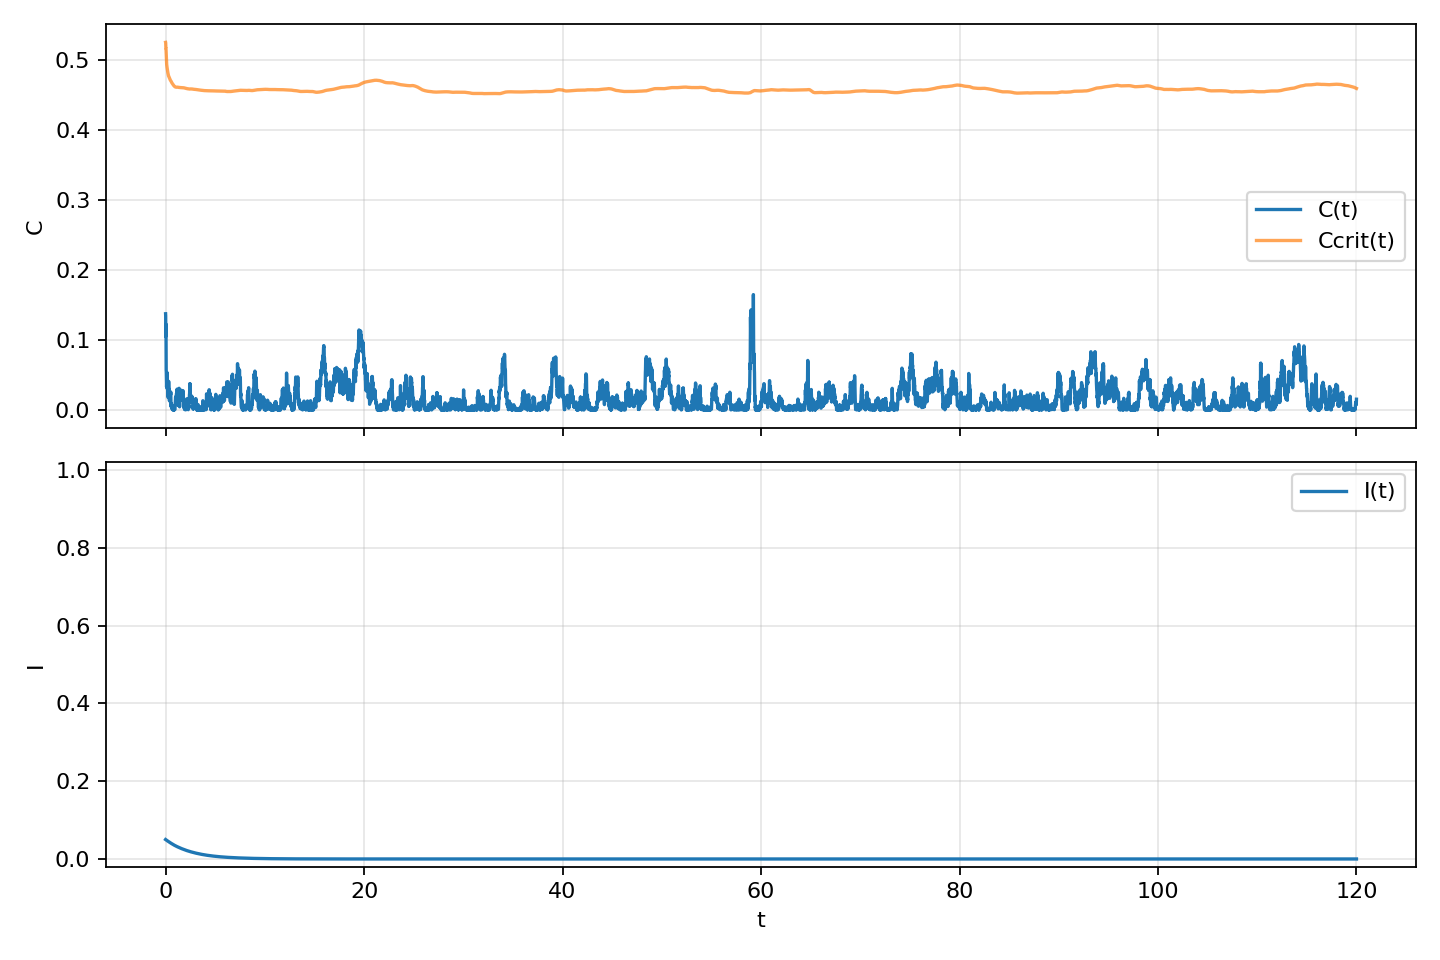
\includegraphics[width=0.85\linewidth]{figures/CI_stable.png}
    \caption{Stable regime: $C(t)$ remains below $C_{\mathrm{crit}}(t)$ and $I(t)$ stays near zero.}
    \label{fig:ci_stable}
\end{figure}

\end{document}




